% ============================================================
% SYNOPSIS
% STATE AWARE RETRIEVAL FOR ITERATIVE RAG
%
% COMPILER:
% pdfLaTeX
%
% OPTIONAL FILES USED WHEN AVAILABLE:
% image1.png
% gantt_chart.png
% ============================================================

\documentclass[12pt,a4paper]{report}

% ============================================================
% FONT
% ============================================================

\usepackage{newtxtext,newtxmath}

% ============================================================
% PAGE SIZE AND MARGINS
% ============================================================

\usepackage[
    a4paper,
    top=0.66in,
    bottom=0.66in,
    left=0.78in,
    right=0.78in
]{geometry}

% ============================================================
% PACKAGES
% ============================================================

\usepackage{setspace}
\usepackage{graphicx}
\usepackage{array}
\usepackage{booktabs}
\usepackage{longtable}
\usepackage{tabularx}
\usepackage{ragged2e}
\usepackage{amsmath}
\usepackage{tikz}
\usepackage{eso-pic}
\usepackage{fancyhdr}
\usepackage{tocloft}
\usepackage{hyperref}
\usepackage{enumitem}
\usepackage{float}
\usepackage[table]{xcolor}
\usepackage{etoolbox}

\makeatletter
\patchcmd{\thebibliography}
  {\chapter*{\bibname}}
  {}
  {}
  {}
\makeatother

% ============================================================
% GENERAL FORMATTING
% ============================================================

\setlength{\parindent}{0pt}
\setlength{\parskip}{0pt}
\onehalfspacing

\hypersetup{
    colorlinks=false,
    hidelinks
}

% ============================================================
% PAGE BORDER
% ============================================================

\AddToShipoutPictureBG{%
    \begin{tikzpicture}[remember picture,overlay]
        \draw[line width=0.5pt]
        ([xshift=0.30in,yshift=-0.30in]current page.north west)
        rectangle
        ([xshift=-0.30in,yshift=0.30in]current page.south east);
    \end{tikzpicture}%
}

% ============================================================
% HEADER / FOOTER
% ============================================================

\pagestyle{fancy}
\fancyhf{}

\fancyhead[R]{%
    \raisebox{0.22in}{%
        \fontsize{10}{12}\selectfont
        Department of Computer Engineering
    }%
}

\fancyfoot[C]{%
    \raisebox{0.18in}{%
        \fontsize{10}{12}\selectfont
        \thepage
    }%
}

\renewcommand{\headrulewidth}{0pt}
\renewcommand{\footrulewidth}{0pt}
\setlength{\headheight}{15pt}

\fancypagestyle{plain}{
    \fancyhf{}
    \fancyhead[R]{%
        \raisebox{0.22in}{%
            \fontsize{10}{12}\selectfont
            Department of Computer Engineering
        }%
    }
    \fancyfoot[C]{%
        \raisebox{0.18in}{%
            \fontsize{10}{12}\selectfont
            \thepage
        }%
    }
    \renewcommand{\headrulewidth}{0pt}
    \renewcommand{\footrulewidth}{0pt}
}

% ============================================================
% TITLE COMMANDS
% ============================================================

\newcommand{\fronttitle}[1]{
    \begin{center}
        {\fontsize{18}{21}\selectfont\bfseries #1\par}
    \end{center}
    \vspace{0.12in}
}

\newcommand{\chaptertitle}[2]{
    \begin{center}
        {\fontsize{18}{21}\selectfont\bfseries CHAPTER #1\par}
        \vspace{0.10in}
        {\fontsize{18}{21}\selectfont\bfseries #2\par}
    \end{center}
    \vspace{0.12in}
}

% ============================================================
% DOCUMENT
% ============================================================

\begin{document}

% ============================================================
% PAGE 1 -- TITLE PAGE
% ============================================================

\begin{titlepage}
\thispagestyle{empty}
\begin{center}

\vspace*{0.58in}

{\fontsize{16}{19}\selectfont\bfseries
SAR: State Aware Retrieval\\for Iterative Retrieval Augmented Generation\par}

\vspace{0.18in}

{\fontsize{12}{18}\selectfont
A Synopsis report submitted in\par}
\vspace{0.12in}
{\fontsize{12}{18}\selectfont
partial fulfillment of requirements for the degree of\par}
\vspace{0.12in}
{\fontsize{12}{18}\selectfont
Bachelor of Technology\par}
\vspace{0.10in}
{\fontsize{12}{18}\selectfont\bfseries\itshape
In\par}
\vspace{0.08in}
{\fontsize{12}{18}\selectfont
Computer Engineering\par}
\vspace{0.10in}
{\fontsize{12}{18}\selectfont\bfseries\itshape
By\par}
\vspace{0.08in}
{\fontsize{12}{18}\selectfont
Kunal Dahal (22CSEC17)\par
Aniket Manger (22CSEC23)\par
Suman Chettri (22CSEC44)\par}

\vspace{0.10in}

{\fontsize{12}{18}\selectfont\itshape
Under the supervision of\par}
\vspace{0.06in}
{\fontsize{14}{17}\selectfont\bfseries
Mr. Anmol Pandey\par}
\vspace{0.04in}
{\fontsize{12}{18}\selectfont
Assistant Professor\par}
\vspace{0.04in}
{\fontsize{12}{18}\selectfont
Computer Engineering Department\par}
\vspace{0.12in}

\IfFileExists{image1.png}{
\includegraphics[width=0.82in]{image1.png}}{\fbox{\rule{0pt}{0.82in}\rule{0.82in}{0pt}}}

\vspace{0.10in}
{\fontsize{14}{17}\selectfont\bfseries
Department Of Computer Engineering\par}
\vspace{0.04in}
{\fontsize{14}{17}\selectfont\bfseries
Sikkim Institute of Science and Technology\par}
\vspace{0.04in}
{\fontsize{14}{17}\selectfont\bfseries
(A constituent college of Sikkim University)\par}
\vspace{0.04in}
{\fontsize{14}{17}\selectfont\bfseries
2026\par}

\end{center}
\end{titlepage}

% ============================================================
% START ROMAN PAGE NUMBERING
% ============================================================

\pagenumbering{roman}
\setcounter{page}{1}

% ------------------------------------------------------------
% ABSTRACT
% ------------------------------------------------------------

\pagenumbering{roman}
\fronttitle{ABSTRACT}
\justifying

Retrieval-Augmented Generation (RAG) combines information retrieval with
large language models so that answers can be supported by information
from external documents. This is especially useful for complex questions
whose required evidence may be distributed across multiple documents.
However, when retrieval is performed iteratively, selecting documents
only on the basis of their relevance to the original question may cause
the system to retrieve information that has already been covered instead
of information that is still required.

This project is going to study and develop a \textbf{Gap-Aware Retrieval (GAR)}
approach for iterative RAG. The proposed approach is going to consider the
current question, the information that is still missing, and the evidence
that has already been collected when selecting documents for the next
retrieval step. The project is going to focus on reducing redundant
retrieval and improving the selection of complementary evidence for
complex question answering. A mathematical formulation for the retrieval
state and a document-scoring equation is going to be developed as part of
the project; no final equation has been established at the synopsis stage.
The proposed retrieval approach is then going to be integrated into the
existing iterative RAG setting and evaluated through systematic
experiments.

\textbf{Keywords:} Retrieval-Augmented Generation, Information Retrieval,
Gap-Aware Retrieval, Iterative Retrieval, Missing Information, Evidence
Retrieval, Multi-Hop Question Answering.

\clearpage

% ============================================================
% PAGE 3 -- TABLE OF CONTENTS
% ============================================================

\fronttitle{TABLE OF CONTENTS}
\begin{center}
\renewcommand{\arraystretch}{1.45}
\makebox[\textwidth][c]{%
\begin{tabular}{|>{\centering\arraybackslash}p{0.55in}|
                >{\centering\arraybackslash}p{5.5in}|
                >{\centering\arraybackslash}p{0.55in}|}
\hline
\textbf{SL NO.} & \textbf{TOPICS} & \textbf{PAGE NO.} \\
\hline
& ABSTRACT & i \\
\hline
1. & INTRODUCTION & 1 \\
\hline
2. & LITERATURE SURVEY & 2--6 \\
\hline
3. & PROBLEM DEFINITION & 7 \\
\hline
4. & OBJECTIVES & 8 \\
\hline
5. & APPLICATIONS & 9 \\
\hline
6. & GANTT CHART & 10 \\
\hline
7. & REFERENCES & 11 \\
\hline
\end{tabular}%
}
\end{center}
\clearpage

% ============================================================
% PAGE 4 -- LISTS
% ============================================================

\fronttitle{LIST OF TABLES}
\begin{center}
\renewcommand{\arraystretch}{1.45}
\makebox[\textwidth][c]{%
\begin{tabular}{|>{\centering\arraybackslash}p{1.0in}|
                >{\centering\arraybackslash}p{4.8in}|
                >{\centering\arraybackslash}p{1.0in}|}
\hline
\textbf{TABLE NO.} & \textbf{TITLE} & \textbf{PAGE NO.} \\
\hline
2.1 & Literature Survey 1 & 2 \\
\hline
2.2 & Literature Survey 2 & 3 \\
\hline
2.3 & Literature Survey 3 & 4 \\
\hline
2.4 & Literature Survey 4 & 5 \\
\hline
2.5 & Literature Survey 5 & 6 \\
\hline
\end{tabular}%
}
\end{center}

\vspace{0.35in}
\fronttitle{LIST OF FIGURES}
\begin{center}
\renewcommand{\arraystretch}{1.45}
\makebox[\textwidth][c]{%
\begin{tabular}{|>{\centering\arraybackslash}p{1.0in}|
                >{\centering\arraybackslash}p{4.8in}|
                >{\centering\arraybackslash}p{1.0in}|}
\hline
\textbf{FIGURE NO.} & \textbf{TITLE} & \textbf{PAGE NO.} \\
\hline
6.1 & Gantt Chart & 10 \\
\hline
\end{tabular}%
}
\end{center}
\clearpage

% ------------------------------------------------------------
% INTRODUCTION
% ------------------------------------------------------------

\pagenumbering{arabic}
\setcounter{page}{1}

\fronttitle{1. INTRODUCTION}
\justifying

Retrieval-Augmented Generation (RAG) is a framework in which a language
model retrieves relevant information from an external document collection
and uses that information to generate an answer. By supplying external
evidence at generation time, RAG extends a language model beyond the
information contained only in its parameters and is therefore useful for
knowledge-intensive question answering \cite{lewis2020rag}. The central
role of the retrieval stage is to select a small set of documents that can
provide the evidence required to answer the question \cite{lewis2020rag}.

The first additional work considered in this project is the work of
Izacard and Grave, which uses multiple retrieved passages with a
generative model. Its findings show that an answer can depend on useful
information distributed across several retrieved passages rather than on
a single passage alone \cite{izacard2021fid}. This indicates that retrieval
quality is not only about finding one highly relevant document, but also
about obtaining a useful collection of evidence \cite{izacard2021fid}.
Yadav et al. further studied iterative evidence retrieval for multi-hop
question answering. Their work shows that later retrieval steps can be
guided by information that has not yet been covered by the evidence
already collected \cite{yadav2020iterative}. This suggests that the
retrieval requirement can change after each retrieval step \cite{yadav2020iterative}.

Wang et al. introduced MIGRES, a missing-information-guided iterative
framework in which the system identifies what information is still missing
after evidence has been collected and uses that information to guide the
next retrieval step \cite{wang2025migres}. Thus, the retrieval process can
maintain an evolving state consisting of what is already known and what is
still required \cite{wang2025migres}. Pickett et al. studied Relevant
Information Gain and emphasized selecting information that adds useful
content while avoiding unnecessary redundancy with information already
retrieved \cite{pickett2024better}. Their work therefore provides a basis
for considering the amount of new information contributed by a candidate
document \cite{pickett2024better}.

From these findings, the problem discovered in the present project is that
a conventional relevance-based retrieval decision may remain focused on
the original question even after part of the required information has
already been obtained. In an iterative setting, this can cause later
retrieval steps to return documents that are related to the question but
overlap with existing evidence, while documents containing complementary
or still-missing information may receive less attention. The issue is
therefore not simply whether a document is relevant to the question, but
whether it is useful with respect to the current information gap and the
evidence already collected.

To address this problem, the project is going to introduce
\textbf{Gap-Aware Retrieval (GAR)} as a reranking component within the
iterative RAG setting. The project is going to use the existing MIGRES
process to provide the current information gap and previously collected
evidence, while GAR is going to focus on selecting the most useful
documents from the retrieved candidate set. The proposed approach is
going to consider three directions: relevance to the question and current
gap, coverage of the missing information, and novelty with respect to
previous evidence. A mathematical formulation for combining these
signals is going to be developed during the project; no final equation is
being claimed at the synopsis stage.

The proposed approach is expected to reduce redundant retrieval and help
later retrieval steps focus on complementary evidence that is still needed.
It is also going to be evaluated for its effect on retrieval quality and
downstream question answering within the iterative RAG pipeline.
\clearpage

% CHAPTER 2 -- LITERATURE SURVEY
% ============================================================

\addcontentsline{toc}{chapter}{2. LITERATURE SURVEY}
\chaptertitle{2}{LITERATURE SURVEY}
\small

% ------------------------------------------------------------
% PAPER 1
% ------------------------------------------------------------
\begin{center}\textbf{Table 2.1: Literature Survey 1}\end{center}
\begin{longtable}{|p{1.25in}|p{5.15in}|}
\hline
\textbf{Name of paper} & Retrieval-Augmented Generation for Knowledge-Intensive NLP Tasks \\ \hline

\textbf{Authors} & Patrick Lewis, Ethan Perez, Aleksandra Piktus, Fabio Petroni, Vladimir Karpukhin, Naman Goyal, Heinrich K\"uttler, Mike Lewis, Wen-tau Yih, Tim Rockt\"aschel, Sebastian Riedel, and Douwe Kiela \\ \hline

\textbf{Publication Details} & Advances in Neural Information Processing Systems 33 (NeurIPS), 2020, pp. 9459--9474. \\ \hline

\textbf{Research Findings} &
\begin{itemize}[leftmargin=0.18in,itemsep=0.05in,topsep=0pt,parsep=0pt]
\item RAG combines information stored in a language model with information retrieved from external documents.
\item Retrieved passages help the model answer questions that require outside knowledge.
\item The approach shows that retrieval can improve the performance of language generation for knowledge-intensive tasks.
\item The work provides a basic foundation for modern retrieval-augmented generation systems.
\end{itemize} \\ \hline

\textbf{Research Gap} &
\begin{itemize}[leftmargin=0.18in,itemsep=0.05in,topsep=0pt,parsep=0pt]
\item The main retrieval process is based on finding passages relevant to the given question.
\item It does not mainly focus on identifying which information is still missing after previous evidence has been retrieved.
\item The work does not specifically study how retrieval can change according to the information already collected.
\end{itemize} \\ \hline

\textbf{Relevance with Our Work} &
\begin{itemize}[leftmargin=0.18in,itemsep=0.05in,topsep=0pt,parsep=0pt]
\item This paper provides the basic RAG background for our project.
\item It supports the use of external documents to provide additional information to language models.
\item Our work builds on this general retrieval setting by studying retrieval in a more iterative information-seeking process.
\end{itemize} \\ \hline
\end{longtable}
\clearpage


% ------------------------------------------------------------
% PAPER 2
% ------------------------------------------------------------
\begin{center}\textbf{Table 2.2: Literature Survey 2}\end{center}
\begin{longtable}{|p{1.25in}|p{5.15in}|}
\hline

\textbf{Name of paper} & Leveraging Passage Retrieval with Generative Models for Open Domain Question Answering \\ \hline

\textbf{Authors} & Gautier Izacard and Edouard Grave \\ \hline

\textbf{Publication Details} & Proceedings of the 16th Conference of the European Chapter of the Association for Computational Linguistics (EACL), 2021, pp. 874--880. \\ \hline

\textbf{Research Findings} &
\begin{itemize}[leftmargin=0.18in,itemsep=0.05in,topsep=0pt,parsep=0pt]
\item The method retrieves multiple passages and provides them to a generative model.
\item The model can use information from several passages to answer a question.
\item Using useful information from multiple retrieved passages can improve question-answering performance.
\item The work shows the importance of selecting and using several relevant pieces of evidence.
\end{itemize} \\ \hline

\textbf{Research Gap} &
\begin{itemize}[leftmargin=0.18in,itemsep=0.05in,topsep=0pt,parsep=0pt]
\item The focus is mainly on how a generative model uses multiple retrieved passages.
\item It does not mainly study how the retrieval process should identify information that is missing from earlier evidence.
\item The retrieved passages are not selected according to a changing information state across multiple retrieval steps.
\end{itemize} \\ \hline

\textbf{Relevance with Our Work} &
\begin{itemize}[leftmargin=0.18in,itemsep=0.05in,topsep=0pt,parsep=0pt]
\item This work supports the importance of collecting multiple useful pieces of evidence.
\item It is indirectly related to our goal of improving the usefulness of retrieved documents.
\item Our project further considers how the current information need can be used when selecting documents during iterative retrieval.
\end{itemize} \\ \hline
\end{longtable}
\clearpage


% ------------------------------------------------------------
% PAPER 3
% ------------------------------------------------------------
\begin{center}\textbf{Table 2.3: Literature Survey 3}\end{center}
\begin{longtable}{|p{1.25in}|p{5.15in}|}
\hline

\textbf{Name of paper} & LLMs Know What They Need: Leveraging a Missing Information Guided Framework to Empower Retrieval-Augmented Generation \\ \hline

\textbf{Authors} & Keheng Wang, Feiyu Duan, Peiguang Li, Sirui Wang, and Xunliang Cai \\ \hline

\textbf{Publication Details} & Proceedings of the 31st International Conference on Computational Linguistics (COLING), 2025, pp. 2379--2400. \\ \hline

\textbf{Research Findings} &
\begin{itemize}[leftmargin=0.18in,itemsep=0.05in,topsep=0pt,parsep=0pt]
\item MIGRES identifies information that is still missing after processing the retrieved evidence.
\item The identified missing information is used to guide the next retrieval step.
\item The framework performs retrieval and evidence processing in multiple steps.
\item The approach is designed for questions that require several pieces of information.
\end{itemize} \\ \hline

\textbf{Research Gap} &
\begin{itemize}[leftmargin=0.18in,itemsep=0.05in,topsep=0pt,parsep=0pt]
\item The framework mainly focuses on identifying missing information and guiding the next retrieval query.
\item There is still room to study how candidate documents can be ranked using both the missing information and the evidence already collected.
\item Different document-ranking strategies may affect which evidence is selected during the iterative process.
\end{itemize} \\ \hline

\textbf{Relevance with Our Work} &
\begin{itemize}[leftmargin=0.18in,itemsep=0.05in,topsep=0pt,parsep=0pt]
\item MIGRES provides an important background for understanding missing information during iterative RAG.
\item It supports the idea that later retrieval should focus on information that is still required.
\item Our project uses this general idea as motivation for studying a gap-aware retrieval and reranking approach.
\item The paper provides the main framework in which our proposed approach can be investigated.
\end{itemize} \\ \hline
\end{longtable}
\clearpage


% ------------------------------------------------------------
% PAPER 4
% ------------------------------------------------------------
\begin{center}\textbf{Table 2.4: Literature Survey 4}\end{center}
\begin{longtable}{|p{1.25in}|p{5.15in}|}
\hline

\textbf{Name of paper} & Unsupervised Alignment-based Iterative Evidence Retrieval for Multi-hop Question Answering \\ \hline

\textbf{Authors} & Vikas Yadav, Steven Bethard, and Mihai Surdeanu \\ \hline

\textbf{Publication Details} & Proceedings of the 58th Annual Meeting of the Association for Computational Linguistics (ACL), 2020, pp. 4514--4525. \\ \hline

\textbf{Research Findings} &
\begin{itemize}[leftmargin=0.18in,itemsep=0.05in,topsep=0pt,parsep=0pt]
\item AIR is an iterative method designed to retrieve evidence for multi-hop questions.
\item The retrieval process changes after each step instead of using the same query throughout.
\item Later retrieval focuses on information that is not already covered by the available evidence.
\item The work shows that iterative retrieval can help collect complementary evidence.
\end{itemize} \\ \hline

\textbf{Research Gap} &
\begin{itemize}[leftmargin=0.18in,itemsep=0.05in,topsep=0pt,parsep=0pt]
\item The method mainly focuses on changing the retrieval query based on previously collected information.
\item It does not fully explore a separate ranking stage that considers relevance, missing information, and existing evidence together.
\item There is room to investigate other ways of selecting complementary documents during iterative retrieval.
\end{itemize} \\ \hline

\textbf{Relevance with Our Work} &
\begin{itemize}[leftmargin=0.18in,itemsep=0.05in,topsep=0pt,parsep=0pt]
\item AIR is closely related to the idea of avoiding already-covered information.
\item It supports the importance of retrieving complementary evidence in multi-step question answering.
\item This provides useful background for studying a retrieval method that considers the current information state.
\end{itemize} \\ \hline
\end{longtable}
\clearpage

% ------------------------------------------------------------
% PAPER 5
% ------------------------------------------------------------
\begin{center}\textbf{Table 2.5: Literature Survey 5}\end{center}
\begin{longtable}{|p{1.25in}|p{5.15in}|}
\hline

\textbf{Name of paper} & Better RAG using Relevant Information Gain \\ \hline

\textbf{Authors} & Marc Pickett, Jeremy Hartman, Ayan Kumar Bhowmick, Raquib-ul Alam, and Aditya Vempaty \\ \hline

\textbf{Publication Details} & arXiv preprint, 2024, arXiv:2407.12101. \\ \hline

\textbf{Research Findings} &
\begin{itemize}[leftmargin=0.18in,itemsep=0.05in,topsep=0pt,parsep=0pt]
\item The paper studies how relevant information gain can be used to improve document selection in RAG.
\item It aims to reduce redundant information while keeping the retrieved information relevant.
\item The approach gives importance to documents that provide useful information not already present in the selected evidence.
\item The work highlights the importance of balancing relevance with the usefulness of new information.
\end{itemize} \\ \hline

\textbf{Research Gap} &
\begin{itemize}[leftmargin=0.18in,itemsep=0.05in,topsep=0pt,parsep=0pt]
\item The main focus is on selecting useful and non-redundant information from retrieved passages.
\item It does not mainly focus on a changing information need across several retrieval steps.
\item The current missing information can provide an additional signal for deciding which document should be selected next.
\end{itemize} \\ \hline

\textbf{Relevance with Our Work} &
\begin{itemize}[leftmargin=0.18in,itemsep=0.05in,topsep=0pt,parsep=0pt]
\item This work provides useful background for reducing repeated or unnecessary evidence.
\item It supports the idea that document selection should consider more than simple relevance.
\item The concept of useful new information is indirectly related to our goal of selecting documents that help cover the current information gap.
\end{itemize} \\ \hline

\end{longtable}
\clearpage

% ============================================================


% CHAPTER 3 -- PROBLEM DEFINITION
% ============================================================

\addcontentsline{toc}{chapter}{3. PROBLEM DEFINITION}
\chaptertitle{3}{PROBLEM DEFINITION}
\justifying

\begin{enumerate}[leftmargin=0.30in,itemsep=0.12in,parsep=0pt]

\item
In iterative Retrieval-Augmented Generation (RAG), some useful information may already be retrieved in earlier steps. However, the next retrieval may return similar information instead of focusing on what is still missing.

\item
In conventional retrieval, documents are mainly selected according to their relevance to the query. This may favor information that has already been collected instead of information that is still missing.

\item
Previous evidence is not fully considered when selecting documents for later retrieval. As a result, redundant documents may be selected while useful and complementary documents may be missed.

\item
Therefore, there is a need for a state aware retrieval approach that considers the query, missing information, and previously collected evidence to select more useful documents for the next retrieval step.

\end{enumerate}
\clearpage


% ============================================================


% CHAPTER 4 -- OBJECTIVES
% ============================================================

\addcontentsline{toc}{chapter}{4. OBJECTIVES}
\chaptertitle{4}{OBJECTIVES}

\begin{enumerate}[leftmargin=0.30in,itemsep=0.12in,parsep=0pt]

\item
To study existing RAG and iterative retrieval methods and identify the limitations of relevance-based retrieval in later retrieval steps.

\item
To study how missing information can be used to guide document retrieval in an iterative setting.

\item
To study how previously collected evidence can be used to reduce redundant information and select complementary documents.

\item
To experimentally evaluate and verify the effectiveness of the proposed Gap-Aware Retrieval (GAR) for improving document retrieval in iterative RAG.

\end{enumerate}
\clearpage


% ============================================================


% ============================================================

% CHAPTER 5 -- APPLICATIONS
% ============================================================

\addcontentsline{toc}{chapter}{5. APPLICATIONS}
\chaptertitle{5}{APPLICATIONS}

\begin{enumerate}[leftmargin=0.30in,itemsep=0.12in]

\item
\textbf{Complex Question Answering:} Can support AI systems in answering complex questions where the required information is spread across multiple documents and cannot be obtained through a single retrieval step.

\item
\textbf{Multi-Step Information Retrieval:} Can be applied to systems that repeatedly search for information, helping each retrieval step focus on information that has not yet been obtained.

\item
\textbf{Research and Knowledge Discovery:} Can assist in collecting information from large document collections by prioritizing useful and complementary evidence instead of repeatedly retrieving similar content.

\item
\textbf{Evidence-Based RAG Applications:} Can be integrated into RAG-based applications where the system needs to build a complete set of evidence before generating an answer, such as question answering, document analysis, and knowledge-based assistants.

\end{enumerate}
\clearpage

% CHAPTER 6 -- GANTT CHART
% ============================================================

\addcontentsline{toc}{chapter}{6. GANTT CHART}
\chaptertitle{6}{GANTT CHART}
\begin{center}
\textbf{Figure 6.1: Gantt Chart}
\vspace{0.15in}

\IfFileExists{gantt_chart.png}{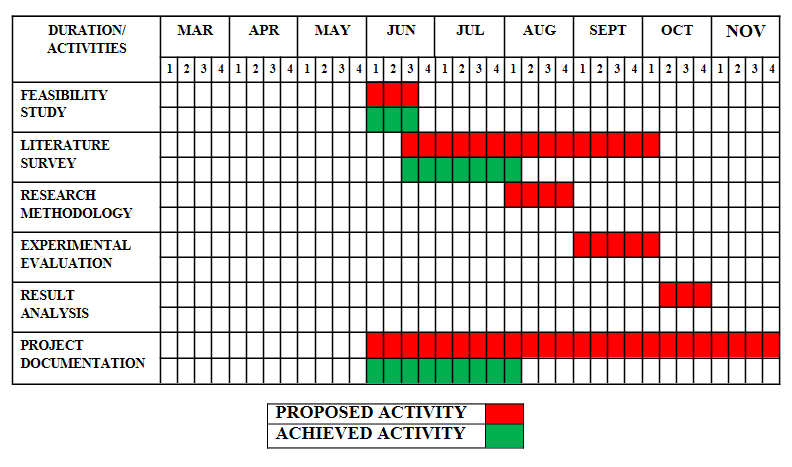
\includegraphics[width=0.95\textwidth]{gantt_chart.png}}{%
\fbox{\parbox[c][3.1in][c]{0.90\textwidth}{\centering Gantt chart image to be inserted here.}}
}
\end{center}
\clearpage

% ============================================================
% CHAPTER 7 -- REFERENCES
% ============================================================

\addcontentsline{toc}{chapter}{7. REFERENCES}
\chaptertitle{7}{REFERENCES}
\renewcommand{\bibname}{}
\bibliographystyle{IEEEtran}
\nocite{*}
\bibliography{citation}

\end{document}